\documentclass[tikz,border=2pt]{standalone}
\usepackage{amsmath}
\usepackage{amssymb}
\usepackage{pgfplots}
\pgfplotsset{compat=1.18}
\usetikzlibrary{arrows.meta}
\begin{document}
% Complete unravelling: theta ~ U[0,1], u(theta) = theta, w(theta) = 3/2 theta. Buyers value an offered
% car at E[w | theta <= p] = 3p/4 for 0 < p <= 1 and 3/4 for p > 1, always below the price p, so the
% price falls step by step (1 -> 0.75 -> 0.5625 -> ...) towards 0, a right limit; the conditional mean is undefined at the zero-probability event p = 0.
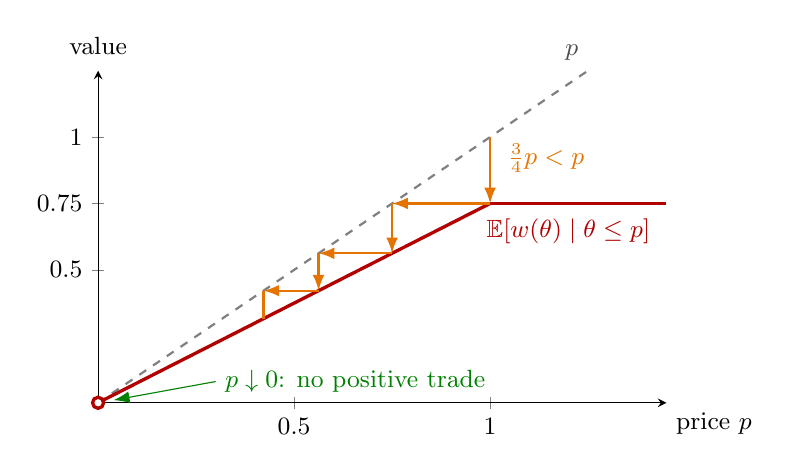
\begin{tikzpicture}[font=\small, >={Latex[length=2mm]}]
  \begin{axis}[
    axis lines=left, xmin=0, xmax=1.45, ymin=0, ymax=1.25,
    xtick={0.5,1}, ytick={0.5,0.75,1},
    xlabel={price $p$}, ylabel={value},
    ylabel style={rotate=-90, anchor=south, at={(axis description cs:0,1.02)}},
    xlabel style={anchor=north west, at={(axis description cs:1.0,0.0)}},
    width=8.8cm, height=5.8cm, clip=false]
    % 45-degree line: the price itself
    \addplot[gray, thick, dashed, domain=0:1.25, samples=2] {x};
    \node[gray!60!black, anchor=south east] at (axis cs:1.25,1.25) {$p$};
    % buyers' value of a car offered at price p
    \addplot[red!70!black, very thick, domain=0:1, samples=2] {0.75*x};
    \addplot[red!70!black, very thick, domain=1:1.45, samples=2] {0.75};
    \node[red!70!black, anchor=north] at (axis cs:1.2,0.73) {$\mathbb{E}[w(\theta)\mid \theta\le p]$};
    % unravelling staircase
    \draw[orange!90!black, thick, ->] (axis cs:1,1) -- (axis cs:1,0.75);
    \draw[orange!90!black, thick, ->] (axis cs:1,0.75) -- (axis cs:0.75,0.75);
    \draw[orange!90!black, thick, ->] (axis cs:0.75,0.75) -- (axis cs:0.75,0.5625);
    \draw[orange!90!black, thick, ->] (axis cs:0.75,0.5625) -- (axis cs:0.5625,0.5625);
    \draw[orange!90!black, thick, ->] (axis cs:0.5625,0.5625) -- (axis cs:0.5625,0.4219);
    \draw[orange!90!black, thick, ->] (axis cs:0.5625,0.4219) -- (axis cs:0.4219,0.4219);
    \draw[orange!90!black, thick] (axis cs:0.4219,0.4219) -- (axis cs:0.4219,0.3164);
    \node[orange!90!black, anchor=west] at (axis cs:1.02,0.92) {$\tfrac{3}{4} p<p$};
    % Open endpoint: conditional mean is defined only for p > 0.
    \draw[red!70!black, fill=white, very thick] (axis cs:0,0) circle (2pt);
    \draw[green!50!black, thin, ->] (axis cs:0.3,0.08) -- (axis cs:0.04,0.01);
    \node[green!50!black, anchor=west] at (axis cs:0.3,0.08) {$p\downarrow0$: no positive trade};
  \end{axis}
\end{tikzpicture}
\end{document}
